\documentclass[runningheads,a4paper]{llncs}

\usepackage[utf8]{inputenc}
\usepackage[T1]{fontenc}
%\usepackage[ngerman]{babel}
\usepackage{enumerate}
\usepackage{listings}
\usepackage{marvosym}
\usepackage{gensymb}
\usepackage[bookmarks,bookmarksopen,bookmarksdepth=2]{hyperref}
\usepackage{amsmath}
\usepackage{amsfonts}
\usepackage{amssymb}
%\usepackage{amsthm}
\usepackage{mathrsfs}
\usepackage{fancyhdr}

\usepackage{graphicx}
\graphicspath{{./img/}}

\usepackage[acronym,toc]{glossaries}
\makeglossaries

%%%%%%%%%%%%%%%%%%%%%%%%%%%%%%%%%%%%%%%%%%%%%%%%%%%%%%%%%%%%%%%%%%%%%%%%%

%\newtheorem{definition}{Definition}
%\newtheorem{theorem}{Theorem}
\newtheorem{axiom}{Axiom}


\newcommand{\Any}{\textsf{Any}}
\newcommand{\partOf}{~\textsf{partOf}~}
\newcommand{\properPartOf}{~\textsf{properPartOf}~}
\newcommand{\atomOf}{~\textsf{atomOf}~}
\newcommand{\fragmentOf}{~\textsf{fragmentOf}~}
\newcommand{\atomicFragmentOf}{~\textsf{atomicFragmentOf}~}
\newcommand{\correspondsTo}{~\textsf{correspondsTo}~}
\newcommand{\correspondsToR}[1]{~\textsf{correspondsTo}_{#1}~}
\newcommand{\conformsTo}{~\textsf{conformsTo}~}

\newcommand{\footnoteurl}[1]{\footnote{\url{#1}}}

\newcommand{\megal}{\text{MegaL}}
\newcommand{\megalxtext}{\text{MegaL/Xtext}}
\newcommand{\megaltext}{\text{MegaL/Text}}
\newcommand{\eclipse}{\text{eclipse}}
\newcommand{\thesis}{Megamodel-driven Traceability Recovery \& Exploration\\of Correspondence \& Conformance Links}


%%%%%%%%%%%%%%%%%%%%%%%%%%%%%%%%%%%%%%%%%%%%%%%%%%%%%%%%%%%%%%%%%%%%%%%%%

\title{Exposé for B.Sc. Thesis}
\subtitle{\thesis}
\author{Maximilian Meffert\\210101205}
\institute{University of Koblenz-Landau}

\begin{document}


\maketitle
%
%\begin{abstract}
%asdf 
%\end{abstract}


\section{Introduction}
This exposé\footnote{\url{http://www.softlang.org/info:expose}} outlines the thesis:
\begin{center}
\it
\thesis
\end{center}
for acquiring the degree Bachelor Science (B.Sc.) in Computer Science.
The central topic of the thesis will be the study of traceability recovery in a megamodel governed environment.
Furthermore a system for exploring the recovered traceability links will be developed.

\subsection{Road-map}
Section \ref{section:Motivation} motivates the topic of the thesis.
\ref{section:Background} gives a short overview over the necessary background information.
\ref{section:ResearchHypthesesAndQuestions} defines a preliminary hypothesis and formulates the research questions.
\ref{section:Objectives} specifies the important objectives for the thesis.
\ref{section:Methodology} describes the approach and methodology of the thesis.
\ref{section:StructureOfTheThesis} outlines the interim structure of the thesis.


\section{Motivation}
\label{section:Motivation}
A common task during the development of software systems is to persist and serialize a domain model.
For instance, consider a simple ReST-ful web-service where data is stored in a database and served via HTTP in serialized form, e.g. XML.
Given such a system, one can observe correspondences (structural similarities) and conformances (compliance with a definition) between different artifacts, i.e. manifestations of the same domain model.
Figure \ref{figure:ORXCorrespondenceBigPicture} shows a non exhaustive depiction of such relationships in O/R/X scenario.

\begin{figure}[h!]
\centering
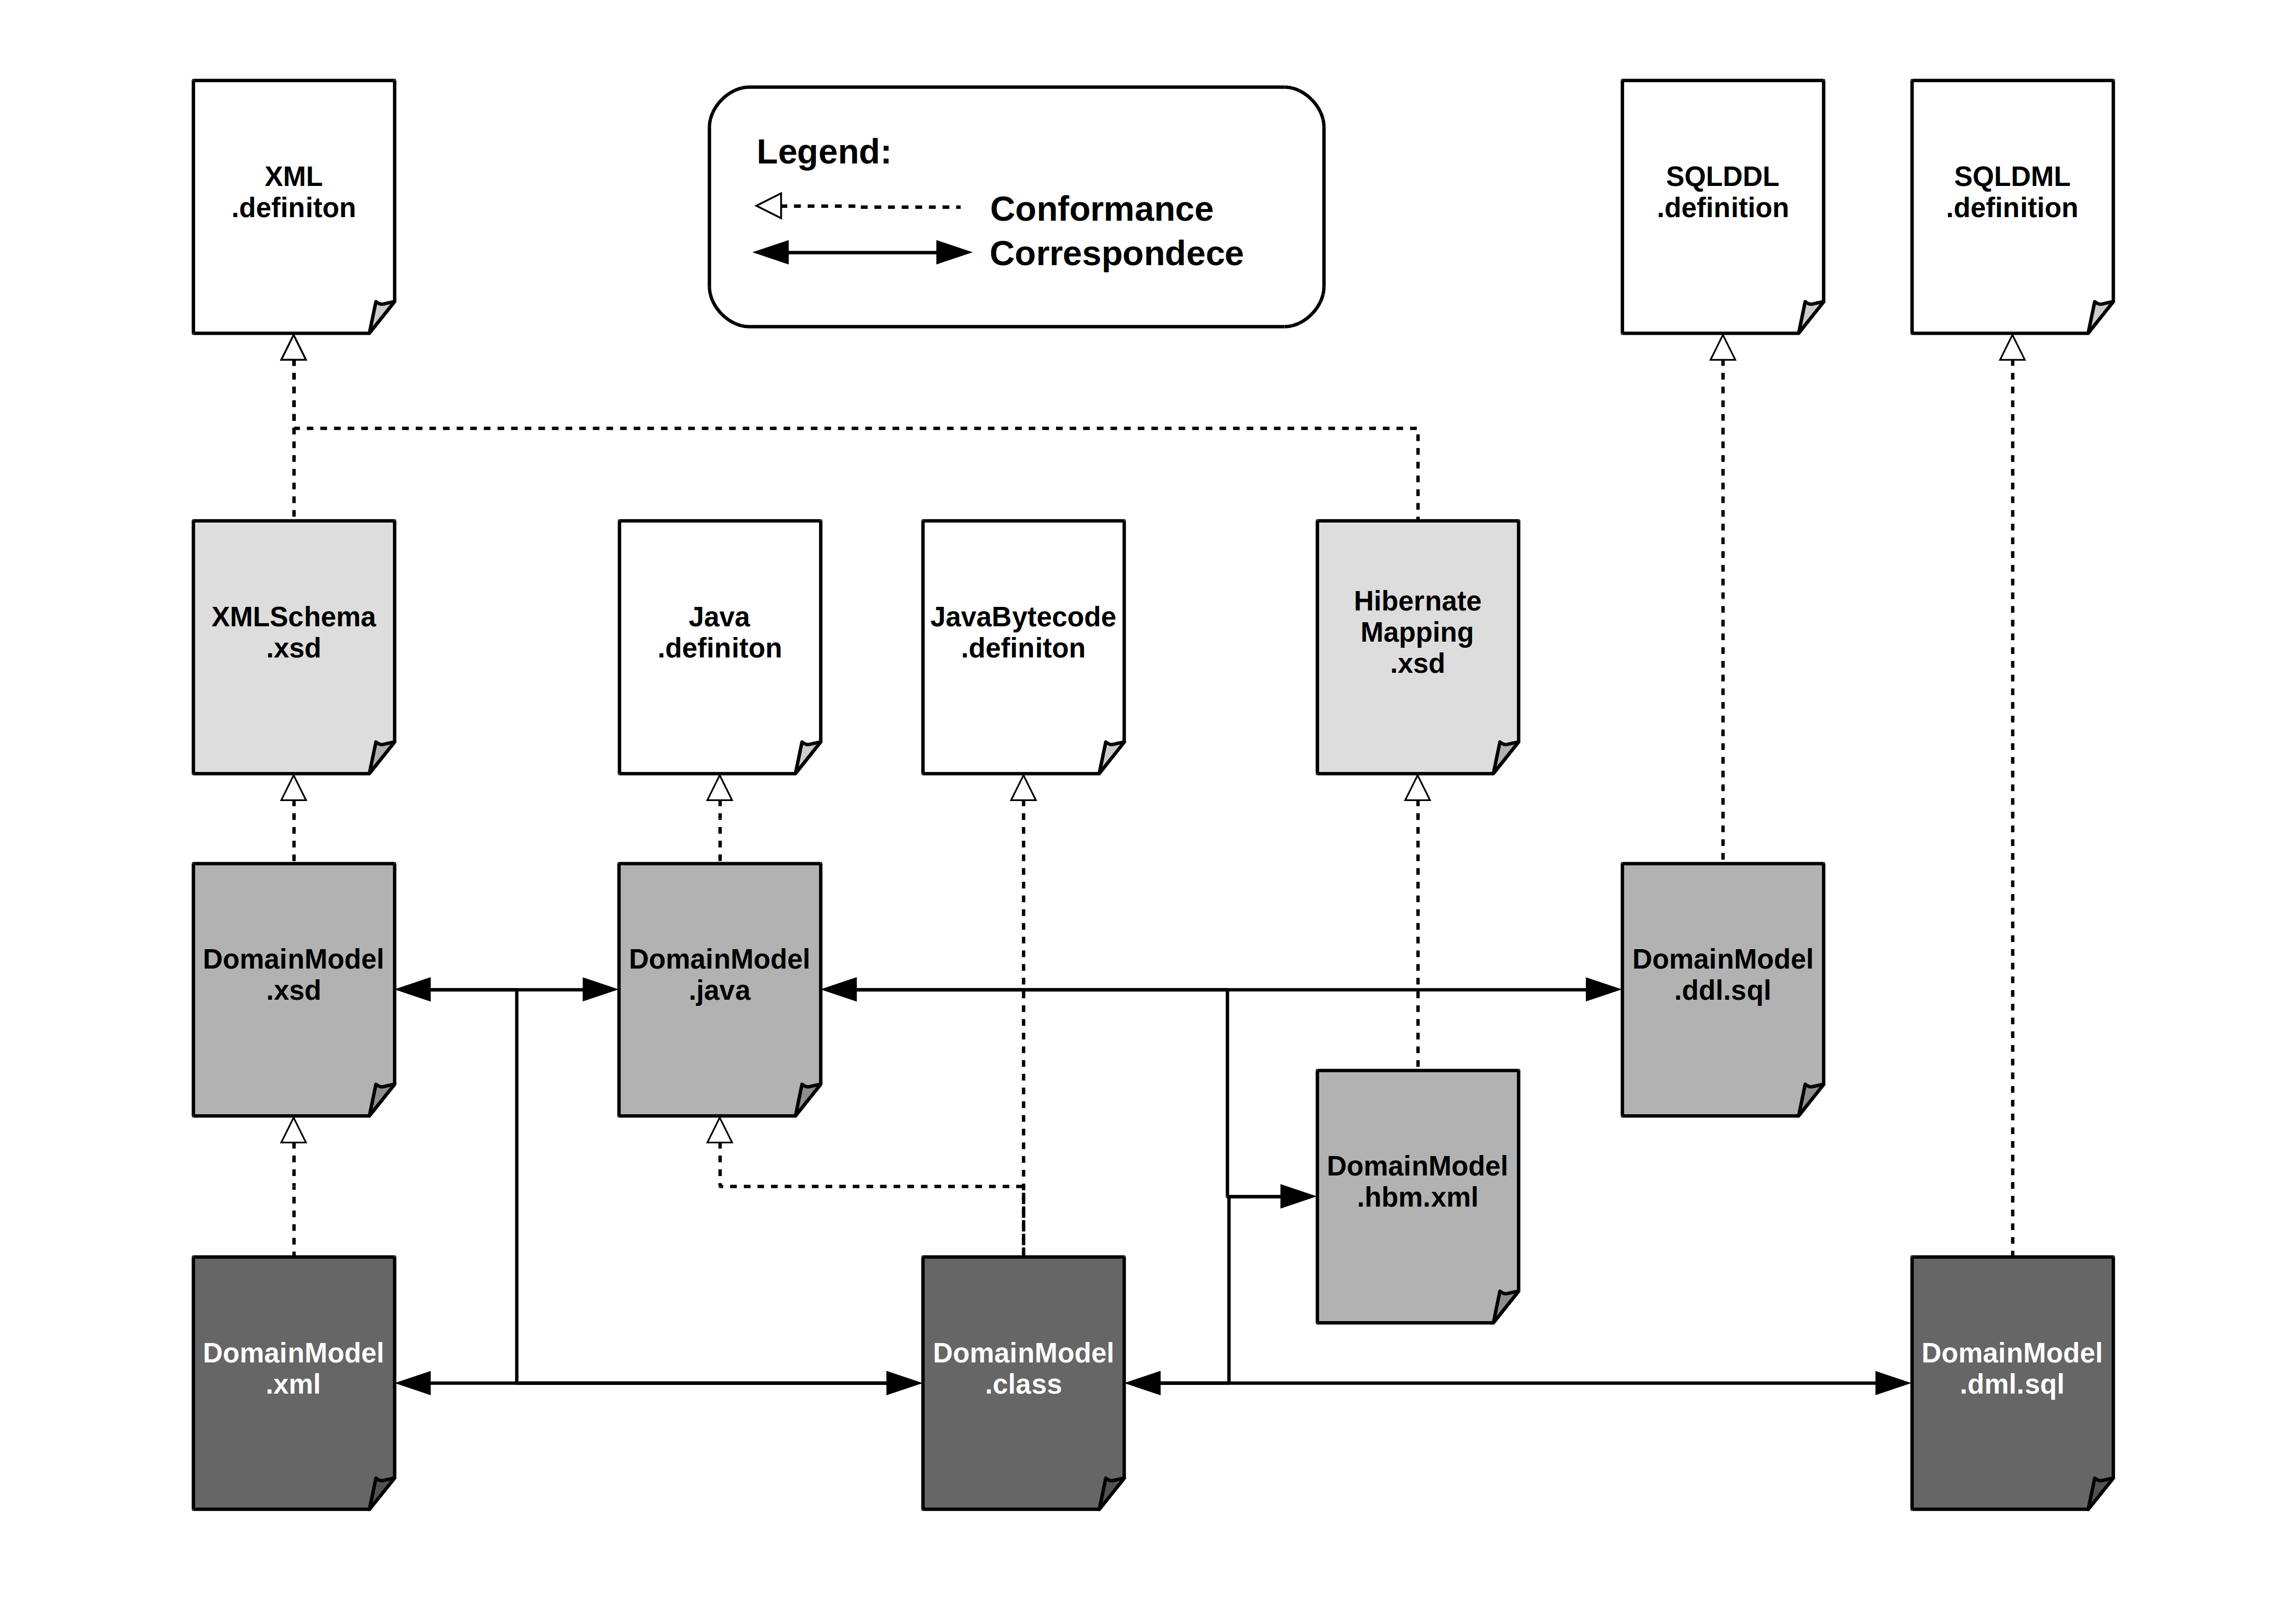
\includegraphics[width=\textwidth]{orx-correspondence-big-picture.png}
\\The depicted relationships may not be exhaustive.
\caption{O/R/X Correspondence \& Conformance}
\label{figure:ORXCorrespondenceBigPicture}
\end{figure}

Upon closer inspection, one can also observe that correspondence and conformance are not just interrelations of the artifacts at large.
In fact the same relations can be found between fragments of the artifacts.
Table \ref{table:ORXCorrespondenceExample} shows fragments corresponding to a Java class property in the O/R/X scenario.

\begin{table}[h!]
\resizebox{\textwidth}{!}{
\begin{tabular}{l|l|l}
\textbf{Language} 
&\textbf{Fragment Type}
&\textbf{Fragment Text}
\\ \hline
Java
&Class Property
&\texttt{public String name;}
\\ \hline
XSD 
&Attribute Definition
&\texttt{<xs:attribute name="name" type="xs:string"/>}
\\ \hline
XML
&Attribute
&\texttt{name="Alan Turing"}
\\ \hline
Hibernate XML
&Property Mapping
&\begin{minipage}{\columnwidth}
\ttfamily
<property access="field" generated="never" lazy="false" name="name" optimistic-lock="true" type="java.lang.String" unique="false">
\\\hspace*{0.05\columnwidth}<column name="name"/>
\\</property>
\end{minipage}
\\ \hline
SQL/DDL
&Column Definition
&\texttt{`name` varchar(255) DEFAULT NULL,}
\\ \hline
SQL/DML
&Column Definition
&\texttt{INSERT INTO Employee (...,name,...) VALUES (...,"Alan Turing",...)}
\end{tabular}
}
\newline
\caption{Corresponding Fragments in an O/R/X Scenario}
\label{table:ORXCorrespondenceExample}
\end{table}

The motivating idea behind the thesis is that correspondence and conformance relationships between artifacts create trace-links left behind by transformations in the sense of \cite{DBLP:conf/sle/Lammel16}.
Thus, it should be possible to recover these links with a model describing such relations.
A technology capable of modeling such \textit{"linguistic architectures"}\cite{DBLP:conf/models/FavreLV12} is $\megal$\footnoteurl{http://www.softlang.org/megal/} \cite{DBLP:conf/ecmdafa/LammelV14}.

\section{Background}
\label{section:Background}
The thesis will be based but is not limited to aspects of the following topics:

\begin{itemize}

\item
\textbf{Traceability}
The ability to interrelate artifacts of a software development process \cite{IEEEGlossary}\cite{Winkler:2010:STR:1861285.1861287}.
The automatic process of relating artifacts is called traceability recovery and recovered elements of the relationships are called links.
Traceability support is one desired capability of $\megal$ and serves as main subject of the thesis.

\item
\textbf{Megamodeling}
The process of interrelating models, e.g. relationships between models, meta-models, meta-meta-models up to meta*-models.
Megamodeling in the sense of $\megal$ mainly interrelates software languages and kindred objects \cite{DBLP:conf/models/FavreLV12}\cite{DBLP:conf/ecmdafa/LammelV14}.

\item
\textbf{Ontologies}
The systematic modeling and representation of knowledge \cite{DBLP:series/ihis/GuarinoOS09}.
Megamodels as used in the thesis are in fact some sorts of software linguistic ontologies, so ontologies may be covered as related work.
Ontologies also utilize mereology.

\item
\textbf{Mereology}
The study of logic part-whole relationships \cite{DBLP:journals/dke/Varzi96}.
Merology serves as theoretical basis for modeling fragments of linguistic artifacts.

\item
\textbf{Program Analysis}
The process of automatically analyzing programs either statically, by analyzing source code, or dynamically by monitoring and intercepting the runtime of a program, i.e. analyzing transient artifacts.
Traceability recovery of linguistic links is in fact an application of program analysis.

\item 
\textbf{XML Data Binding}
The process of automatically mapping model- and instance-level objects into a XML-serialized form.
XML Data Binding as  implemented by JAXB\footnote{Java Architecture for XML Binding \url{https://docs.oracle.com/javase/tutorial/jaxb/intro/arch.html}} will serve as a scenario subjected to traceability recovery of linguistic links.

\item
\textbf{Object Relational Mapping}
The process of automatically mapping model- and instance-level objects into a relational data-storage.
Object Relational Mapping as implemented by JPA\footnote{Java Persistence API \url{http://www.oracle.com/technetwork/articles/javaee/jpa-137156.html}} and Hibernate\footnoteurl{http://hibernate.org/} will serve as another scenario subjected to traceability recovery of linguistic links

\end{itemize}

\section{Research Hypotheses \& Questions}
\label{section:ResearchHypthesesAndQuestions}
Parthood is the relationship between a whole and its constituent parts.
\cite{DBLP:journals/dke/Varzi96} and \cite{DBLP:conf/sle/Lammel16} axiomatize it as a reflexive, antisymmetric and transitive relation:
\begin{align*}
&x \partOf x
\\&x \partOf y \wedge y \partOf x \Rightarrow x = y
\\&x \partOf y \wedge y \partOf z \Rightarrow x \partOf z
\end{align*}
A stricter, irreflexive form of parthood is the proper-part relationship \cite{DBLP:journals/dke/Varzi96}:
\begin{align*}
x \properPartOf y
\Leftrightarrow
x \partOf y \wedge \neg(y \partOf x)
\end{align*}
Since software artifacts are based on formal languages it should also be fair to assume the atomicity axiom \cite{DBLP:journals/dke/Varzi96}:
\begin{align*}
\forall x \exists y : 
y \partOf x \wedge \neg(\exists z : z \properPartOf y)
\end{align*}
Objects with no proper parts are called atoms, otherwise their called fusions.

Correspondence is the relationship between two software artifacts who share a structural similarity.
\cite{DBLP:conf/sle/Lammel16} axiomatizes it as a strict one-to-one relation between software artifacts:
\begin{align*}
&(a_1,a_2) \in R \subseteq L_1 \times L_2
\\&\wedge \forall b_1 \in L_1 : b_1 \partOf a_1 \Rightarrow (\exists! b_2 \in L_2 : b_2 \partOf a_2 \wedge b_1 \correspondsToR{R} b_2 )
\\&\wedge \forall b_2 \in L_2 : b_2 \partOf a_2 \Rightarrow (\exists! b_1 \in L_1 : b_1 \partOf a_2 \wedge b_2 \correspondsToR{R} b_1 )
\\&\Rightarrow a_1 \correspondsToR{R} a_2
\end{align*}

Given an arbitrary relationship $R$ between to languages, for instance a transformation from one language to the other, two artifacts correspond to each other if and only if for each part of one artifact there exists exactly one corresponding part of the other.

Conformance is the relationship between two software artifacts, denoting that one artifact complies to the definition given by the other.
\cite{DBLP:conf/sle/Lammel16} axiomatizes it as follows:
\begin{align*}
\forall x \in \Any :
x \in L \subseteq \Any \Leftrightarrow \exists d \in D \subseteq \Any : x \conformsTo d
\end{align*}

Given a set $\Any$ serving as a universe for software artifacts, an arbitrary artifact conforms to another one if and only if the latter artifact is a definition for software language whom the former is an element of.

One objective of the thesis should be to provide empirical assurance for the axiom above in the sense that correspondence and conformance are in fact to some extend mereologically induced.
However, \cite{DBLP:conf/sle/Lammel16} also notes that strict correspondence may be unrealistic since real world artifacts may contain two or more parts corresponding to only one part in another artifact, e.g. an XSD documents can contain an element and a complex type definition corresponding to only on Java class declaration.
For this reason the thesis will assume a weaker forms of correspondence and conformance as research hypotheses:
\begin{enumerate}[RH1]
\item
\textbf{Fragment Correspondence Hypothesis}
\begin{align*}
&\forall a_1 \in L_1, a_2 \in L_2 \exists b_1 \in L_1, b_2 \in L_2 :  
\\&a_1 \correspondsToR{R} a_2
\Rightarrow 
b_1 \partOf a_2 
\wedge b_2 \partOf a_2
\wedge b_1 \correspondsToR{R} b_2
\end{align*}
If two artifacts are assumed to correspond to each other, then parts of both artifacts should exist which also correspond to each other.

\item
\textbf{Fragment Conformance Hypothesis}
\begin{align*}
&\forall a_1 \in L, a_2 \in D \exists b_1 \in L, b_2 \in D : 
\\&a_1 \conformsTo a_2
\Rightarrow 
b_1 \partOf a_2
\wedge b_2 \partOf a_2
\wedge b_1 \conformsTo b_2
\end{align*}
If two artifacts are assumed to be in a conformance relationship, then parts of both artifacts should exist which share the same relationship.
\end{enumerate}

This leads to the following research questions:
\begin{enumerate}[RQ1]

\item
Is correspondence to some extend strictly mereologically induced?
\begin{align*}
&\forall a_1 \in L_1, a_2 \in L_2 \exists b_1 \in L_1, b_2 \in L_2 :
\\&a_1 \correspondsToR{R} a_2
\\&\Rightarrow 
b_1 \properPartOf a_2 
\wedge b_2 \properPartOf a_2 
\wedge b_1 \correspondsToR{R} b_2
\end{align*}

\item
Is conformance to some extend strictly mereologically induced?
\begin{align*}
&\forall a_1 \in L_1, a_2 \in L_2 \exists b_1 \in L_1, b_2 \in L_2 :
\\&a_1 \conformsTo a_2
\\&\Rightarrow 
b_1 \properPartOf a_2 
\wedge b_2 \properPartOf a_2 
\wedge b_1 \conformsTo b_2
\end{align*}

\end{enumerate}

\section{Objectives}
\label{section:Objectives}
Objectives for the thesis are:
\begin{enumerate}[O1]
\item
Implementation of a \megalxtext-extension capable of recovering traceability links representing parthood, correspondence and conformance relationships between code fragments.

\item
Implementation of a $\megalxtext$-extension allowing for an user to visually explore traceability links, i.e. parthood, correspondence and conformance relationships between code fragments

\item
Providing an extensive discussion comparing $\megal$ with related approaches on traceability recovery.

\item
Providing an extensive discussion comparing $\megal$ with related approaches on ontologies for software artifacts or software engineering in general.

\item
Providing an answer for the research questions.

\end{enumerate}

\section{Methodology}
\label{section:Methodology}
Thesis and research will utilize an example-driven approach inspired by the 101system\footnoteurl{https://101wiki.softlang.org/101system}.
For this, the system to study will be an imaginary Human Resource Management System (HRMS).
Figure \ref{figure:TheCompanyModel} shows an UML-Class-Diagram depicting the model of this system.

\begin{figure}[h!]
\centering
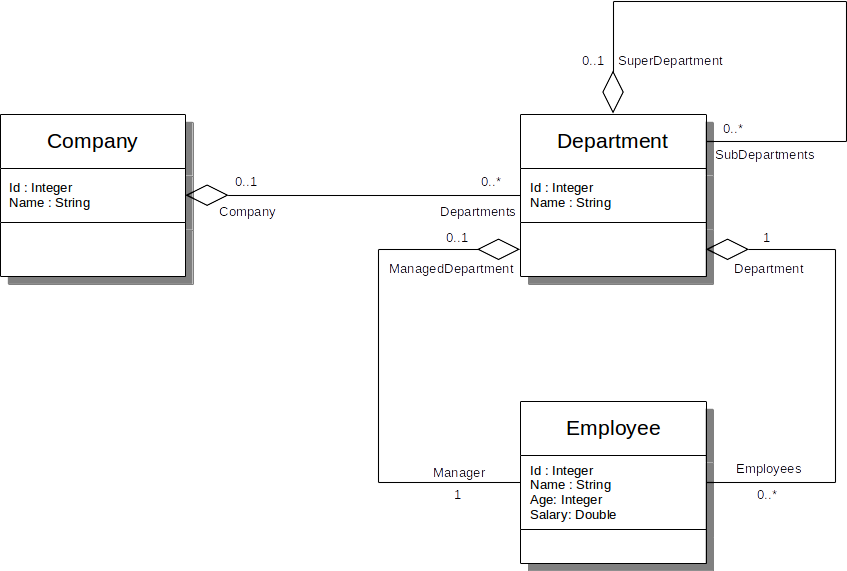
\includegraphics[width=\textwidth]{companies.png}
\caption{The Human Resource Management System Model}
\label{figure:TheCompanyModel}
\end{figure}

The HRMS will be implemented in plain Java with two scenarios in mind:
(a) XML-Binding with JAXB
and (b) Persistence with JPA/Hibernate.
Both scenarios will be studied with the concrete instance of the HRMS model.


\section{Structure of the Thesis}
\label{section:StructureOfTheThesis}
The interim structure\footnoteurl{http://softlang.wikidot.com/info:thesis-structure} of the thesis is outlined by but not limited to the chapters as follows:

\begin{enumerate}

\item
\textbf{Introduction}
This chapter will introduce the thesis subject, also delimiting possible contributions to traceability recovery and megamodeling.

\item
\textbf{Background}
This chapter will provide the theoretical background of the thesis as outlined but not limited to the topics in section \ref{section:Background} above.

\item
\textbf{Related Work}
This chapter will provide a sound discussion of related work regarding megamodeling and traceability recovery of linguistic relationships between software artifacts.

\item
\textbf{Methodology}
This chapter will describe the approach of the thesis as outlined in section \ref{section:Methodology} above.

\item
\textbf{Requirements}
This chapter will define the requirements and acceptance criteria for the system to be developed as described in section \ref{section:Objectives}.

\item
\textbf{Design}
This chapter will provide a description of the design and architecture for the developed system from section \ref{section:Objectives}.

\item
\textbf{Implementation}
This chapter will provide explanations of non trivial implementation details of the developed system, e.g. a fragmentation algorithm for software artifacts could be necessary for the system.

\item
\textbf{Results}
This chapter will provide a discussion of empirical results gathered by the implemented system from section \ref{section:Objectives} applied to the scenarios described in section \ref{section:Methodology}.

\item
\textbf{Conclusion}
This chapter will summarize the thesis, pointing out possible limitations and future work.

\end{enumerate}




%\cite{DBLP:conf/ecmdafa/LammelV14}
%\cite{DBLP:conf/models/FavreLV12}
%\cite{DBLP:journals/dke/Varzi96}
%\cite{DBLP:journals/entcs/FavreN05}
%\cite{Softlang:course/ptt15/technoloymodeling}
%\cite{DBLP:conf/sle/Lammel16}

\bibliographystyle{splncs}
\bibliography{../bsc}{}

%\printglossaries
%\printglossary[type=\acronymtype]

\end{document}
